\section{Types of Policies}
\begin{frame}{}
    \LARGE Policy Search: \textbf{Types of Policies}
\end{frame}

\begin{frame}{Types of Policies}
    \begin{itemize}
        \item Policy $\pi$ determines how the agent chooses actions
        \item Deterministic Policy: $$\pi(s) = a$$
        \item Stochastic Policy: $$\pi(a|s) = Pr(a_t = a | s_t = s)$$
        \item So far have focused on deterministic policies or $\epsilon$-greedy policies
        \item $\epsilon$-greedy policies are also near deterministic as we decrease the value of epsilon with training
        \item Is deterministic policy optimal?
    \end{itemize} 
\end{frame}

\subsection{Example: Aliased Grid world}
\begin{frame}{Example: Aliased Grid world}
    \begin{figure}
        \centering
        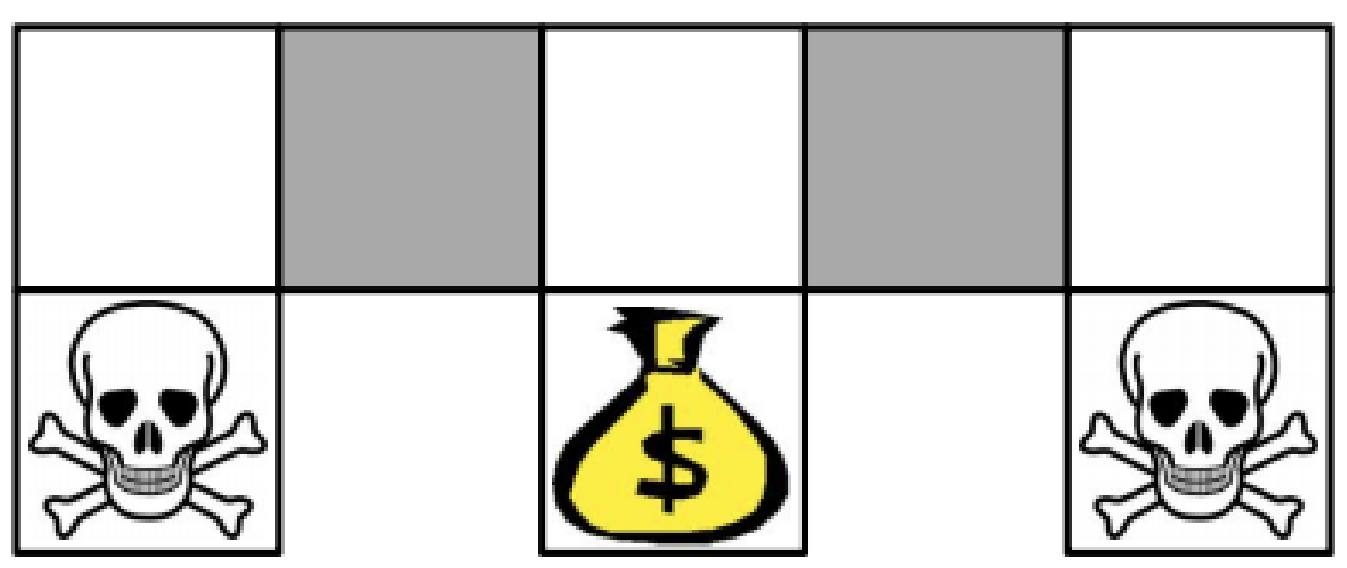
\includegraphics[width=0.9\textwidth,height=0.3\textheight,keepaspectratio]{images/policy-search/grid_world_1.png}
    \end{figure}

    \begin{itemize}
        \item Consider a Grid World as in the image
        \item The agent can move in four direction (N, E, W, S) if valid
        \item The agent \textbf{cannot} differentiate the grey states
    \end{itemize}
\end{frame}

\begin{frame}{Example: Aliased Grid world}
    \begin{figure}
        \centering
        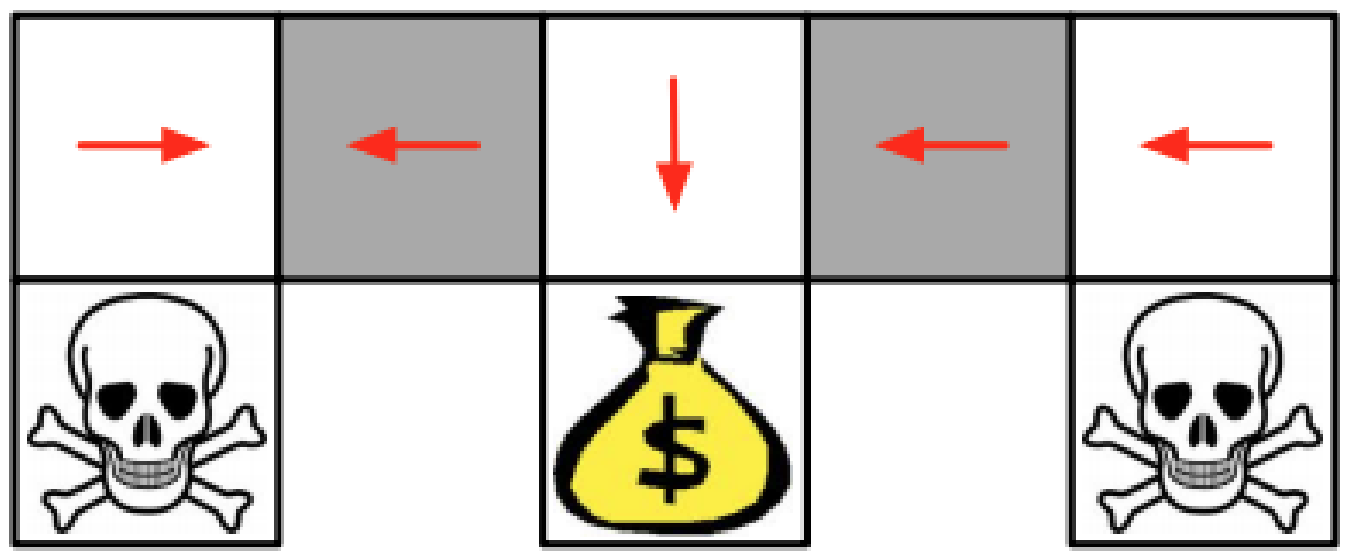
\includegraphics[width=0.9\textwidth,height=0.3\textheight,keepaspectratio]{images/policy-search/grid_world_2.png}
    \end{figure}

    \begin{itemize}
        \item Under aliasing, an optimal deterministic policy will either
        \begin{itemize}
            \item move W in both grey states (shown by red arrows)
            \item move E in both grey states
        \end{itemize}
        \pause
        \item Either way, it can get stuck and never reach the money
        \pause
        \item Similarly, Value-based RL learns a near-deterministic policy (e.g., $\epsilon$-greedy)
        \item As a result, it will traverse the corridor for a long time depending on the value of Epsilon
    \end{itemize}
\end{frame}

    \begin{frame}{Example: Aliased Grid world}
        \begin{figure}
        \centering
        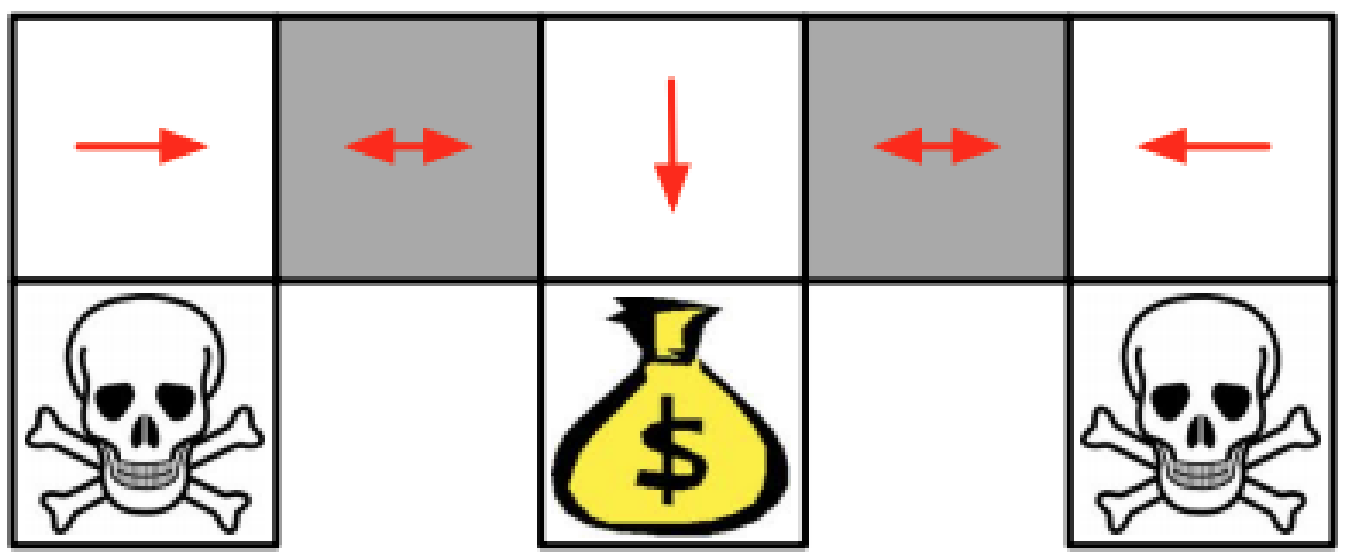
\includegraphics[width=0.9\textwidth,height=0.3\textheight,keepaspectratio]{images/policy-search/grid_world_3.png}
    \end{figure}

    \begin{itemize}
        \item An optimal stochastic policy will randomly move E or W in grey states
        \begin{itemize}
            \item $\pi_\theta$(wall to N and S, move E) = 0.5
            \item $\pi_\theta$(wall to N and S, move W) = 0.5
        \end{itemize}
        \pause
        \item It will reach the goal state in a few steps with high probability
        \pause
        \item Policy-based RL can learn the optimal stochastic policy
    \end{itemize}
\end{frame}